\documentclass[11pt]{article}
\usepackage{cs170}
\usepackage{tikz}

\def\title{Homework 12}
\def\duedate{Monday 4/22/2024, at 10:00 pm (grace period until 11:59pm)}

\begin{document}
\maketitle


Due \textbf{\duedate}

\question{Study Group}
List the names and SIDs of the members in your study group.
If you have no collaborators, you must explicitly write ``none''.

\begin{solution} I worked on this homework with the following collaborators:
\begin{itemize}
    \item Lakshya Nagal, SID: 3037935253
\end{itemize}
\end{solution}

\newpage

\question{Approximating Independent Set}

In the maximum independent set (MIS) problem, we are given a graph $G = (V, E)$, and our goal is to find the largest set of vertices such that no two vertices in the set are connected by an edge. For this problem, we will assume the degree of all vertices in $G$ is bounded by $d$ (i.e. $\forall v \in V, \text{ deg}(v) \leq d$).

Consider the following greedy algorithm to approximate the maximum independent set:

\begin{algorithm}
\begin{algorithmic}[1]
\Procedure{Greedy-MIS}{$V, E$}
\State $I \gets \emptyset$
\While {$G \neq \emptyset$}
\State choose a vertex $v$ in $G$
\State $I = I \cup \{ v \}$
\State remove $v$ and all its neighbors from $G$
\EndWhile
\State return $I$
\EndProcedure
\end{algorithmic}
\end{algorithm}

\begin{subparts}
    \item Provide an example where the greedy approximation does not give the optimal solution.
    \begin{solution}
        Suppose we choose a vertex $v$ such that $deg(v)=d$ and $\forall u \in neighbors(v),~ deg(u)=1$ (i.e none of the neighbors are adjacent to each other). Then we would 
        have been better off excluding vertex $v$ from set $I$ and adding $neighbors(v)$ to set $I$.\\
        \begin{center}
            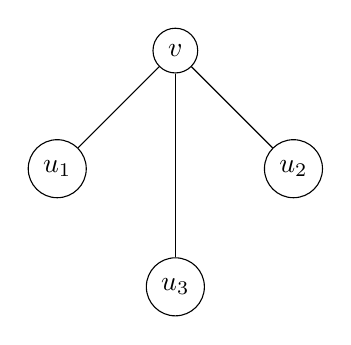
\begin{tikzpicture}[scale=1.5]
                % Nodes
                \node[circle, draw] (center) at (0,0) {$v$};
                \node[circle, draw] (node1) at (-1,-1) {$u_1$};
                \node[circle, draw] (node2) at (1,-1) {$u_2$};
                \node[circle, draw] (node3) at (0,-2) {$u_3$};
                
                % Edges
                \draw (center) -- (node1);
                \draw (center) -- (node2);
                \draw (center) -- (node3);
            \end{tikzpicture}
        \end{center}
    \end{solution}
    \item Provide an approximation ratio for the given greedy algorithm in terms of $|V|$, $|E|$, and/or $d$. Briefly justify your answer. \\
    \begin{solution}
        For the greedy algorithm, $|I|$ is at least $\frac{|V|}{d+1}$ since at every iteration we are removing at most $(d + 1)$ vertices, and for our $OPT(I)$, $|I| = |V|$, applying the ratio
        we get $\frac{|V|}{\frac{|V|}{d+1}} = d + 1$.
    \end{solution}
\end{subparts}

\newpage

\question{$\sqrt{n}$ coloring}
\begin{subparts}
    \subpart \label{part:max-deg-color} Let $G$ be a graph of maximum degree $\delta$.  Show that $G$ is $(\delta+1)$-colorable.\\
    \begin{solution}
        By induction on $n=|V|$, we can show trivially that when $n=1$ we have maximum degree $\delta=0$, and the graph is 
        in fact $(\delta+1)$-colorable. Now assume that for any graph with $n$ vertices and maximum degree $\delta$, the graph is $(\delta + 1)$-colorable. For a graph $G'$ with
        $n+1$ vertices and maximum degree of $\delta$, we can remove a vertex from $G'$ such that the maximum degree is still $\delta$, and under our assumption about a graph with $n$ vertices, $G'-v$ is $(\delta + 1)$-colorable.
        Introducing $v$ back into $G'$ with still a maximum degree $\delta$, we can color $v$ with a different color than its adjacent vertices since we have $\delta + 1$ colors to choose from.       
    \end{solution}
    \subpart \label{part:bipartite-neighborhood} Suppose $G=(V, E)$ is a $3$-colorable graph.  Let $v$ be any vertex in $G$.  Show that the graph induced on the neighborhood of $v$ is $2$-colorable. 
    Note: the graph induced on the neighborhood of $v$ refers to the following subgraph: \[G' = (V'=\text{neighbors of $v$}, E'=\text{all edges in $E$ with both endpoints in $V'$}).\]
    \begin{solution}
        If we are only considering the neighbors of $v$ and their edges and $G$ is 3-colorable, then we have three cases. If the subgraph is disconnected (no edges between the neighbors), trivially it is 2-colorable. if the subgraph
        is a connected component (theres a path from vertex $u$ to $u'$), then we can color each vertex such that we alternate colors. If the subgraph is partially connected (contains some connected components), then we can alternate colors between the connected components of the 
        subgraph.
    \end{solution}
    \subpart \label{part:sqrtn-colors} Give a polynomial time algorithm that takes in a $3$-colorable $n$-vertex graph $G$ as input and outputs a valid coloring of its vertices using $O(\sqrt{n})$ colors.  Prove that your algorithm is correct.
    
    \emph{Hint: think of an algorithm that first assigns colors to ``high-degree'' vertices and their neighborhoods, and then assigns colors to the rest of the graph.  The previous two parts might be useful.}\\
    \begin{solution}
        We can identify all the vertices with high degree in $O(n)$. For each of these vertices we can
        color in the vertices with highest degree and color its neighbors as described in part (b), we can do this in $O(n)$. Then we can go through the 
        graph one more time and assign the other vertices colors such that no two adjacent vertices share the same
        color. In the worst case, we have a graph with $n$ nodes and there is one vertex with maximum degree of $n-1$ and all of 
        its neighbors are adjacent to each other, in this case we would need at most $O(\sqrt{n})$ colors.
    \end{solution}
\end{subparts}

\newpage

\question{Multiway Cut}
In the multiway cut problem, we are given a graph $G=(V, E)$ with $k$ special vertices $s_1, s_2, \ldots, s_k$. Our goal is to find the smallest set of edges $F$ which, when removed from the graph, disconnect the graph into at least $k$ components, where each $s_i$ is in a different component. When $k = 2$, this is exactly the min $s$-$t$ cut problem, but if $k \geq 3$ the problem becomes NP-hard.

Consider the following algorithm: Let $F_i$ be the set of edges in the minimum cut with $s_i$ on one side and all other special vertices on the other side. Output $F$, the union of all $F_i$. Note that this is a multiway cut because removing $F_i$ from $G$ isolates $s_i$ in its own component.

\begin{subparts}
\subpart Explain how each $F_i$ can be found in polynomial time.\\
\begin{solution}
    We can add a vertex to all other special vertex $s_j \not = s_i$ with a capacity of $\infty$. In this way $F_i$ is the min-cut between
    $s_i$ and this newly added vertex. We can we can find in polynomial time.
\end{solution}
\subpart Let $F^*$ be the smallest multiway cut. Consider the components that removing $F^*$ disconnects $G$ into, and let $C_i$ be the set of vertices in the component with $s_i$. Let $F_i^*$ be the set of edges in $F^*$ with exactly one endpoint in $C_i$. How many different $F_i^*$ does each edge in $F^*$ appear in? Which is larger: $F_i$ and $F_i^*$? \\
\begin{solution}
    If we have $k$ special vertices $s_1, s_2, \ldots, s_k$. Each edge in the smallest multiway cut $F^*$ connects two distinct components, one containing $s_i$ and one containing $s_j$ ($i \neq j$). So, each edge in $F^*$ appears in exactly two sets $F_i^*$ and $F_{i^{'}}^*$ (one for each of the two components it connects). Therefore 
    each edge in $F^*$ appears in exactly two of the sets $F_i^*$.
\end{solution}
\subpart Using your answer to the previous part, show that $|F| \leq 2|F^*|$.\\
\begin{solution}
    By the previous part, each edge in $F^*$ appears in exactly two sets $F_i^*$. Therefore, the total number of edges in $F$ is at most twice the total number of edges in $F^*$, $|F| \leq 2|F^*|$.
\end{solution}
\subpart \textbf{Extra Credit:} how could you modify this algorithm to output $F$ such that $|F| \leq (2-\frac{2}{k})|F^*|$?
\end{subparts}

\newpage

\question{Relaxing Integer Linear Programs}

As discussed in lecture, Integer Linear Programming (ILP) is \textsf{NP}-complete. In this problem, we discuss attempts to approximate ILPs with Linear Programs and the potential shortcomings of doing so.

Throughout this problem, you may use the fact that the ellipsoid algorithm finds an optimal vertex (and corresponding optimal value) of a linear program in polynomial time.

\begin{enumerate}[(a)]
    \item Suppose that $\vec{x}_0$ is an optimal point for the following arbitrary LP:
    \begin{align*}
        \text{maximize } &\, c^\top x \\
        \text{subject to: }& Ax\le b \\
        & x\ge 0
    \end{align*} Show through examples (i.e. by providing specific canonical-form LPs and optimal points) why we cannot simply (1) round all of the element in $\vec{x}_0$, or (2) take the floor of every element of $\vec{x}_0$ to get good integer approximations.\\
    \begin{solution}
        Let's say we have the following LP:
        \[
        \begin{aligned}
        \text{maximize } &\, x_1 + x_2 \\
        \text{subject to: } & x_1 + x_2 \leq 2 \\
        & x_1, x_2 \geq 0
        \end{aligned}
        \]
        with optimal solution $\vec{x}_0 = (1.5, 0.5)$.

        \begin{enumerate}[(1)]
            \item Rounding all elements in $\vec{x}_0$ would give us $(2, 1)$, but this violates the constraint $x_1 + x_2 \leq 2$, leading to an infeasible solution.            
            \item Taking the floor of every element of $\vec{x}_0$ would give us $(1, 0)$, which is feasible but is a suboptimal solution. 
        \end{enumerate}

        So rounding or taking the floor of every element in $\vec{x}_0$ doesn't guarantee good approximations due to violating constraints or producing suboptimal solutions.
    \end{solution}
    \item The \textsc{Matching} problem is defined as follows: given a graph $G$, determine the size of the largest subset of disjoint edges of the graph (i.e. edges without repeating incident vertices).

    Find a function $f$ such that:
    \begin{align*}
        \text{maximize } &\, f \\
        \text{subject to:}& \sum_{e\in E, v\in e} x_e \le 1 \qquad \forall v \in V\\
                          & 0 \leq x_e \leq 1 \qquad \forall e \in E
    \end{align*}
    is an LP relaxation of the \textsc{Matching} problem. Note that the ILP version (which directly solves \textsc{Matching}) simply replaces the last constraint with $x_e\in\{0,1\}$.\\
    \begin{solution}
        $f = \sum_{e \in E} x_e$
    \end{solution}
    \item It turns out that the polytope of the linear program from part (b) has vertices whose coordinates are all in $\{0,\frac{1}{2}, 1\}$. Using this information, describe an algorithm that approximates \textsc{Matching} and give an approximation ratio with proof.

    \emph{Hint: round up, then fix constraint violations.}\\
    \begin{solution}
        We solve LP relaxation problem from part (b) and obtain the optimal solution. We can round or solutions
        as follows: if $x_e = \frac{1}{2}$ we round to 1. If any there are any constraint violations, for example say we have 3 edges all connected to 4 vertices and all rounded up to 1, then we can 
        arbitrarily select one edge and set the others to 0 so that no two edges share a vertex. Consider the case where we have 4 vertices and 3 edges $v_1 \leftrightarrow v_2 \leftrightarrow v_3 \leftrightarrow v_4$, and our algorithm selects
        edges $(v_1, v_2), (v_2, v_3)$, then we would need to ignore one of those edges and our solution would consist of only 1 edge. In the optimal solution, however, we would have choosen 2 edges.
        this means that the our algorithms solution is less than optimal solution by a factor of 1/2, giving us a 2-approximation.
    \end{solution}
    \item There is a class of linear program constraints whose polytopes have only integral coordinates. Let $\mathcal{P}_{>2,\text{odd}}(V)$ be the set of subsets of the vertices with size that is odd and greater than 2. It turns out that, if we simply add to the LP from part (b) the following constraints:
    \[\sum_{e\in E(S)}x_e\le \frac{|S|-1}{2}\qquad \forall S\subseteq \mathcal{P}_{>2,\text{odd}}(V),\] then all vertices of the new polytope are integral. First, interpret this constraint in words and explain why it still describes the \textsc{Matching} problem. Then, explain what this result implies about approximating ILPs with (special) LPs. \\
    \begin{solution}
        The constraint is stating that for any subset $S$ that has an odd size and has more than two elements in it, the sum of $x_e$ over all the edges in $S$, is less than or equal 
        to $\frac{|S|-1}{2}$. This is essentially putting a limit on the number of edges within the subset, to prevent from including 
        an extra edge that could be violate the \textsc{Matching} problems constraints. The constraint above  still describes
        the \textsc{Matching} problem since the constraint only helps enforce the fact that more any matching, we don't include more than
        edge that contains vertices already within that set. What this implies about approximating ILP's with special LP's is that we can still obtain a reasonable solution without the use of use of more complicated constraints and rounding schemes.

    \end{solution}
    \item Why doesn't the observation in part (d) imply that \textsc{Matching} $\in \textsf{P}$?\\
    \begin{solution}
        Since formulating and solving an LP as described, can not be done in polynomial time (we would have to check every possible subset $S$ i.e. exponential). Therefore, \textsc{Matching} $\not \in$ P.
    \end{solution}
\end{enumerate}

\end{document}